\documentclass[11pt,compress,t,notes=noshow]{beamer}
\usepackage[]{graphicx}\usepackage[]{color}
% maxwidth is the original width if it is less than linewidth
% otherwise use linewidth (to make sure the graphics do not exceed the margin)
\makeatletter
\def\maxwidth{ %
  \ifdim\Gin@nat@width>\linewidth
    \linewidth
  \else
    \Gin@nat@width
  \fi
}
\makeatother

\definecolor{fgcolor}{rgb}{0.345, 0.345, 0.345}
\newcommand{\hlnum}[1]{\textcolor[rgb]{0.686,0.059,0.569}{#1}}%
\newcommand{\hlstr}[1]{\textcolor[rgb]{0.192,0.494,0.8}{#1}}%
\newcommand{\hlcom}[1]{\textcolor[rgb]{0.678,0.584,0.686}{\textit{#1}}}%
\newcommand{\hlopt}[1]{\textcolor[rgb]{0,0,0}{#1}}%
\newcommand{\hlstd}[1]{\textcolor[rgb]{0.345,0.345,0.345}{#1}}%
\newcommand{\hlkwa}[1]{\textcolor[rgb]{0.161,0.373,0.58}{\textbf{#1}}}%
\newcommand{\hlkwb}[1]{\textcolor[rgb]{0.69,0.353,0.396}{#1}}%
\newcommand{\hlkwc}[1]{\textcolor[rgb]{0.333,0.667,0.333}{#1}}%
\newcommand{\hlkwd}[1]{\textcolor[rgb]{0.737,0.353,0.396}{\textbf{#1}}}%
\let\hlipl\hlkwb

\usepackage{framed}
\makeatletter
\newenvironment{kframe}{%
 \def\at@end@of@kframe{}%
 \ifinner\ifhmode%
  \def\at@end@of@kframe{\end{minipage}}%
  \begin{minipage}{\columnwidth}%
 \fi\fi%
 \def\FrameCommand##1{\hskip\@totalleftmargin \hskip-\fboxsep
 \colorbox{shadecolor}{##1}\hskip-\fboxsep
     % There is no \\@totalrightmargin, so:
     \hskip-\linewidth \hskip-\@totalleftmargin \hskip\columnwidth}%
 \MakeFramed {\advance\hsize-\width
   \@totalleftmargin\z@ \linewidth\hsize
   \@setminipage}}%
 {\par\unskip\endMakeFramed%
 \at@end@of@kframe}
\makeatother

\definecolor{shadecolor}{rgb}{.97, .97, .97}
\definecolor{messagecolor}{rgb}{0, 0, 0}
\definecolor{warningcolor}{rgb}{1, 0, 1}
\definecolor{errorcolor}{rgb}{1, 0, 0}
\newenvironment{knitrout}{}{} % an empty environment to be redefined in TeX

\usepackage{alltt}
\newcommand{\SweaveOpts}[1]{}  % do not interfere with LaTeX
\newcommand{\SweaveInput}[1]{} % because they are not real TeX commands
\newcommand{\Sexpr}[1]{}       % will only be parsed by R



\usepackage[english]{babel}
\usepackage{dsfont}
\newcommand\bmmax{2}
\usepackage{bm}
\usepackage{bbm}
\usepackage{verbatim}
\usepackage{amsmath}
\usepackage{amsfonts}
\usepackage{csquotes}
\usepackage{multirow}
\usepackage{longtable}
\usepackage{enumerate}
\usepackage[absolute,overlay]{textpos}
\usepackage{psfrag}
\usepackage{algorithm}
\usepackage{algorithmicx}
\usepackage{algpseudocode}
\usepackage{eqnarray}
\usepackage{multimedia}
\usepackage{media9}
\usepackage{arydshln}
\usepackage{tabularx}
\usepackage{placeins}
\usepackage{tikz}
\usepackage{setspace}
\usepackage{wrapfig}
\usepackage{tcolorbox}
\usepackage[export]{adjustbox}
\usepackage{siunitx}
\usetikzlibrary{shapes,arrows,automata,positioning,calc}
\def\signed #1{{\leavevmode\unskip\nobreak\hfil\penalty50\hskip1em
  \hbox{}\nobreak\hfill #1%
  \parfillskip=0pt \finalhyphendemerits=0 \endgraf}}

\newsavebox\mybox
\newenvironment{aquote}[1]
  {\savebox\mybox{#1}\begin{quote}\openautoquote\hspace*{-.7ex}}
  {\unskip\closeautoquote\vspace*{1mm}\signed{\usebox\mybox}\end{quote}}
  
\tikzset{
  %Define standard arrow tip
  >=stealth',
  %Define style for boxes
  punkt/.style={
    rectangle,
    rounded corners,
    draw=black, very thick,
    text width=6.5em,
    minimum height=2em,
    text centered},
  % Define arrow style
  pil/.style={
    ->,
    thick,
    shorten <=2pt,
    shorten >=2pt,}
}
\usepackage{subfig}

%new environments

\newenvironment{vbframe}  %frame with breaks and verbatim
{
 \begin{frame}[containsverbatim,allowframebreaks]
}
{
\end{frame}
}

\newenvironment{vframe}  %frame with verbatim without breaks (to avoid numbering one slided frames)
{
 \begin{frame}[containsverbatim]
}
{
\end{frame}
}

\newenvironment{blocki}[1]   % itemize block
{
 \begin{block}{#1}\begin{itemize}
}
{
\end{itemize}\end{block}
}

\newenvironment{fragileframe}[2]{  %fragile frame with framebreaks
\begin{frame}[allowframebreaks, fragile, environment = fragileframe]
\frametitle{#1}
#2}
{\end{frame}}


\newcommand{\myframe}[2]{  %short for frame with framebreaks
\begin{frame}[allowframebreaks]
\frametitle{#1}
#2
\end{frame}}

\newcommand{\remark}[1]{
  \textbf{Remark:} #1
}

%%%%%%%%%%%%%%%%%%%%%%%%%%%%%%%%%%%%%%%%%%%%%%%%%%%%%%%%%%%%%%%%%%%%%%%%%%%%%%%

% basic latex stuff
\newcommand{\pkg}[1]{{\fontseries{b}\selectfont #1}} %fontstyle for R packages
\newcommand{\lz}{\vspace{0.5cm}} %vertical space
\newcommand{\dlz}{\vspace{1cm}} %double vertical space
\newcommand{\oneliner}[1] % Oneliner for important statements
{\begin{block}{}\begin{center}\begin{Large}#1\end{Large}\end{center}\end{block}}


%\usetheme{lmu-lecture}
\usepackage{../style/lmu-lecture}

\let\code=\texttt
\let\proglang=\textsf

\setkeys{Gin}{width=0.9\textwidth}



\title{Introduction to Machine Learning}
\author{Bernd Bischl}
\institute{Department of Statistics -- LMU Munich}
\date{Winter term 2021}

\setbeamertemplate{frametitle}{\expandafter\uppercase\expandafter\insertframetitle}



\begin{document}




\input{../latex-math/basic-math}
\input{../latex-math/basic-ml}
\input{../latex-math/ml-nn}

\lecturechapter{4}{Deep Learning- TrainingX}
\lecture{Deep Learning- TrainingX}
%%%%%%%%%%%%%%%%%%%%%%%%%%%%%%%%%%%%%%%%%%%%%%%%%%%%%%%%%%%%%%%%%%

\begin{vbframe}{Training Neural Networks}
\lz
Training of neural nets is composed of two iterative steps:
\lz
\begin{enumerate}
\item \textbf{Forward pass:} The information of the inputs flow through the model to produce a prediction. Based on that, we compute the empirical loss.
\lz
\item \textbf{Backward pass:} Information of the error of the predictions flows backwards through the model and weights are updated in such a way the error is reduced.
\end{enumerate}
\lz

The error is calculated by a loss function $L(y, f(x, \thetab))$ of the true target $y$ and the networks output $f(x, \thetab)$.
\framebreak
%%%%%%%%%%%%%%%%%%%%%%%%%%%%%%%%%%%%%%%%%%%%%%%%%%%%%%%%%%%%%%%%%%

\begin{itemize}
\item For regression, we typically use the L2 loss:
$$\Lxy = \frac{1}{2}(y - \fx)^2$$
\item For classification we typically apply binary/categorical cross entropy:
$$\Lxy = y \log \fx + (1 - y) \log(1 - \fx)$$
\item Evaluated on the data, we refer to it as the risk function:
$$\riske = \sumin \Lxyi,$$
\end{itemize}
\end{vbframe}
%%%%%%%%%%%%%%%%%%%%%%%%%%%%%%%%%%%%%%%%%%%%%%%%%%%%%%%%%%%%%%%%%%

\begin{vbframe}{Training Neural Networks}
\begin{itemize}
\item To minimize the risk, we need to exploit the method of gradient descent in numerical optimization.
\item At a point $\theta^{[t]}$ we can calculate the gradient $\nabla \risk$, which always points in the direction of the steepest ascent.
\item Thus, $-\nabla \risk$ points in the direction of the steepest descent!

%%%%%%%%%%%%%%%%%%%%%%%%%%%%%%%%%%%%%%%%%%%%%%%%%%%%%%%%%%%%%%%%%%

\item At a point $\theta^{[t]}$ during minimization, we can improve by doing the following step:
\[\thetab^{[t + 1 ]}  = \thetab^{[t]} - \alpha \nabla \risk\left(\thetab^{[t]}\right)\]
where $\alpha$ determines the length of the step and is called learning rate.
\end{itemize}
\framebreak
%%%%%%%%%%%%%%%%%%%%%%%%%%%%%%%%%%%%%%%%%%%%%%%%%%%%%%%%%%%%%%%%%%

\begin{figure}
\scalebox{1}{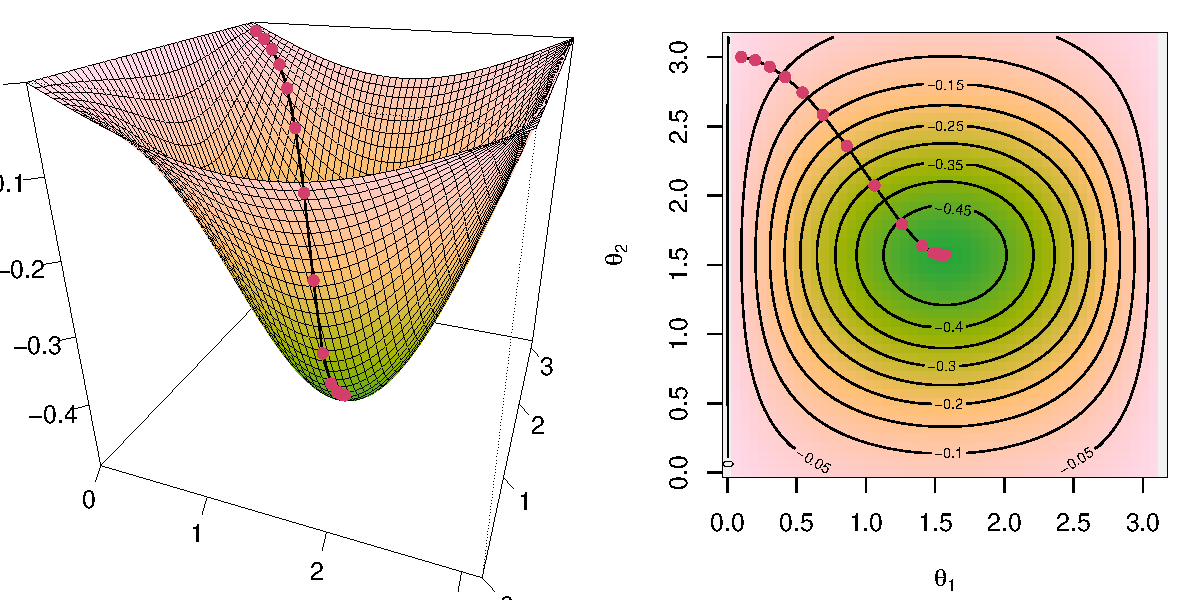
\includegraphics{plots/hill.pdf}}
\end{figure}
\hspace{1cm} Example of gradient descent with $\theta=(w_1, w_2)$: \textit{"Walking down the hill, towards the valley."}
\end{vbframe}
%%%%%%%%%%%%%%%%%%%%%%%%%%%%%%%%%%%%%%%%%%%%%%%%%%%%%%%%%%%%%%%%%%

\begin{vbframe}{Weight updates with Backpropagation}
\begin{itemize}
\item To update each weight $w \in \thetab$ in the network we need their gradients with regards to the risk.
\item Since weights are stacked in layers inside the network, we need to repeatedly apply the *chain rule of calculus*. This process is called \textbf{backpropagation}.
\item After obtaining the gradients we can update the weights by gradient descent
\[\thetab^{[t + 1]} = \thetab^{[t]} - \alpha \cdot \frac{1}{n} \cdot \sumin \nabla_\theta L\left(\yi, f(\xi ~|~ \thetab^{[t]})\right)\]
\end{itemize}
\end{vbframe}
%%%%%%%%%%%%%%%%%%%%%%%%%%%%%%%%%%%%%%%%%%%%%%%%%%%%%%%%%%%%%%%%%%

\begin{vbframe}{Weight updates with Backpropagation}
\begin{itemize}
\item Optimization algorithms that use the entire training set to compute updates in one huge step are called batch or deterministic. This is computationally very costly or often impossible.
\item Instead of letting the sum run over the whole dataset (batch mode) one can also let it run only over small subsets of size $m$ (minibatches).
\item With minibatches of size $m$, a full pass over the training set (called an epoch) consists of $\frac{n}{m}$ gradient updates.
\end{itemize}
\framebreak
%%%%%%%%%%%%%%%%%%%%%%%%%%%%%%%%%%%%%%%%%%%%%%%%%%%%%%%%%%%%%%%%%%

  \begin{algorithm}[H]
  \footnotesize
    \caption{Basic SGD pseudo code}
    \begin{algorithmic}[1]
    \State Initialize parameter vector $\thetab^{[0]}$

    \State $t \leftarrow 0$
    \While{stopping criterion not met}
    \State Randomly shuffle data and partition into minibatches $J_1, ..., J_K$ of size $m$
      \For{$k\in\{1,...,K\}$}
      \State $t \leftarrow t + 1$
      \State Compute gradient estimate with $J_k$:
      \[\hat{g}^{[t]} \leftarrow \frac{1}{m} \sum_{i \in J_k} \nabla_\theta L(\yi, f(\xi ~|~ \thetab^{[t-1]}))
      \]
      \State Apply update: $\thetab^{[t]} \leftarrow \thetab^{[t-1]} - \alpha \hat{g}^{[t]}$

      \EndFor


      \EndWhile
    \end{algorithmic}
  \end{algorithm}
  
\end{vbframe}
%%%%%%%%%%%%%%%%%%%%%%%%%%%%%%%%%%%%%%%%%%%%%%%%%%%%%%%%%%%%%%%%%%

\begin{vbframe}{Weight updates with Backpropagation}
\begin{itemize}
\item While SGD remains a popular optimization strategy, learning with it can sometimes be slow.
\item Momentum is designed to accelerate learning, especially when facing high curvature, small but consistent or noisy gradients:
\begin{eqnarray*}
\nu &\leftarrow& \varphi \nu - \alpha g(\theta) \\
\theta &\leftarrow& \theta + \nu
\end{eqnarray*}
\item Accumulate an exponentially decaying moving average of past gradients.
\end{itemize}
\end{vbframe}
%%%%%%%%%%%%%%%%%%%%%%%%%%%%%%%%%%%%%%%%%%%%%%%%%%%%%%%%%%%%%%%%%%

\begin{vbframe}{SGD with Momentum}
\begin{figure}
\scalebox{.8}{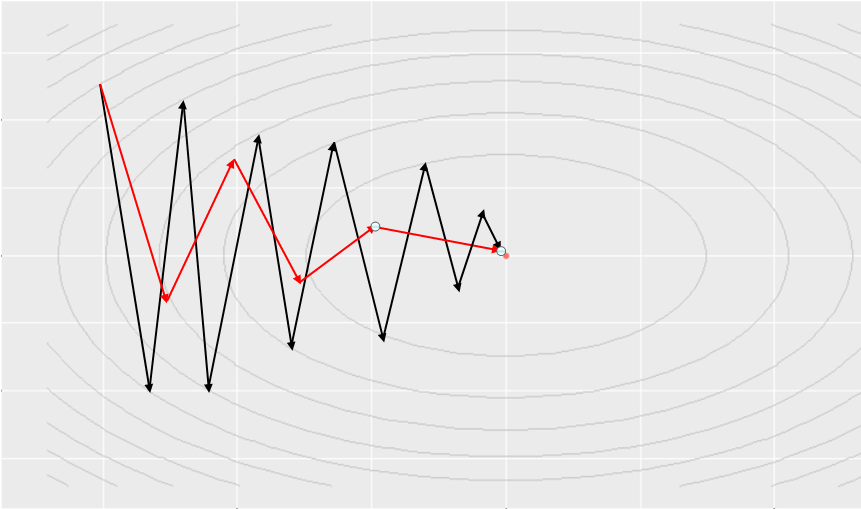
\includegraphics{plots/momentum.png}}
\end{figure}
The contour lines show a quadratic loss function with a poorly conditioned Hessian matrix. The to curves show how standard gradient descent (black) and momentum (red) learn when dealing with ravines.
\end{vbframe}
%%%%%%%%%%%%%%%%%%%%%%%%%%%%%%%%%%%%%%%%%%%%%%%%%%%%%%%%%%%%%%%%%%

\begin{vbframe}{Momentum in Practice}
\begin{figure}
\scalebox{.8}{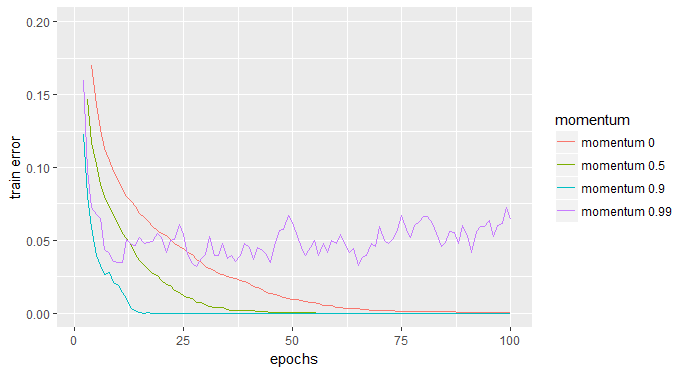
\includegraphics{plots/momentum_train.png}}
\end{figure}
The higher momentum, the faster SGD learns the weights on the training data, but if momentum is too large, the training and test error fluctuates.
\end{vbframe}
%%%%%%%%%%%%%%%%%%%%%%%%%%%%%%%%%%%%%%%%%%%%%%%%%%%%%%%%%%%%%%%%%%

\begin{vbframe}{Early Stopping}
\begin{itemize}
\item When training with an iterative optimizer such as SGD, it is commonly the case that after a certain number of iterations, generalization error begins to increase even though training error continues to decrease.
\item \textbf{Early stopping} refers to stopping the algorithm early, before the generalization error increases.
\end{itemize}
\begin{figure}
\scalebox{.3}{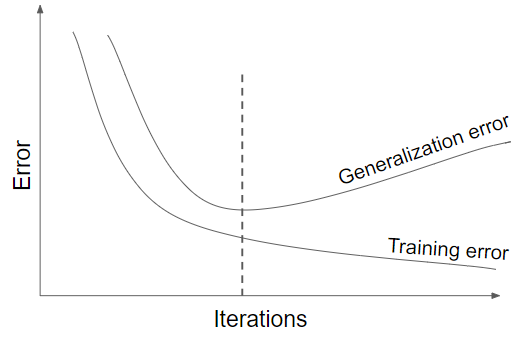
\includegraphics{plots/earlystop.png}}
\end{figure}
After a certain number of iterations, the algorithm begins to overfit.
\framebreak
%%%%%%%%%%%%%%%%%%%%%%%%%%%%%%%%%%%%%%%%%%%%%%%%%%%%%%%%%%%%%%%%%%

\textbf{How early stopping works:}
\begin{enumerate}
\item Split training data $(X^{(train)}, y^{(train)})$ into $(X^{(subtrain)}, y^{(subtrain)})$ and $(X^{(validation)}, y^{(validation)})$ (e.g. with a ratio of 2:1).
\item Use $(X^{(subtrain)}, y^{(subtrain)})$ and evaluate model using the $(X^{(validation)}, y^{(validation)})$.
\item Stop training when validation error stops decreasing (after a range of "patience" steps).
\item Use parameters of the previous step for the actual model.
\end{enumerate}
\framebreak
%%%%%%%%%%%%%%%%%%%%%%%%%%%%%%%%%%%%%%%%%%%%%%%%%%%%%%%%%%%%%%%%%%

\textbf{Strengths:}

\begin{itemize}
\item Effective and simple \& Periodical evaluation of validation error
\item Applicable to almost any model without adjustment
\item Combinable with other regularization methods
\end{itemize}

\textbf{Weaknesses:}

\begin{itemize}
\item Periodical evaluation of validation error
\item Less data for training $\rightarrow$ include $(X^{(validation)}, y^{(validation)})$ afterwards
\end{itemize}

\end{vbframe}
%%%%%%%%%%%%%%%%%%%%%%%%%%%%%%%%%%%%%%%%%%%%%%%%%%%%%%%%%%%%%%%%%%

\begin{vbframe}{Further Regularization Strategies}
\textbf{Parameter penalties}
\begin{itemize}
\item Same as Rigde Regression/L2-Regularization
\item Often referred to as \textit{weight decay} since weights are pulled to zero if they are not updated by large enough values.
\end{itemize}
\begin{figure}
\scalebox{.4}{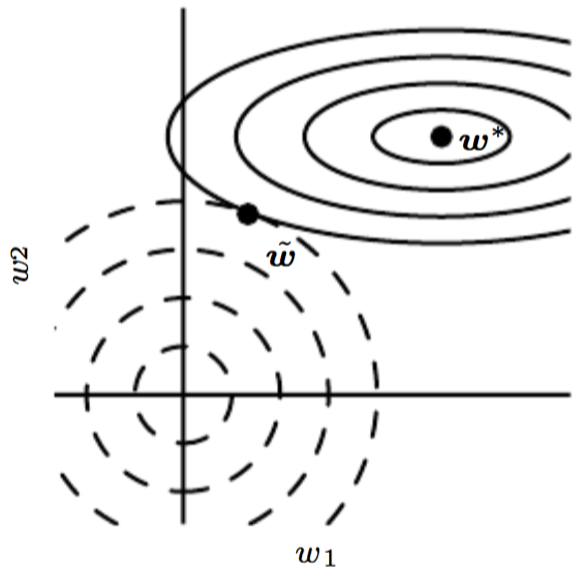
\includegraphics{plots/weight_decay.png}}
\end{figure}
\framebreak
%%%%%%%%%%%%%%%%%%%%%%%%%%%%%%%%%%%%%%%%%%%%%%%%%%%%%%%%%%%%%%%%%%

\textbf{Dropout}
\begin{itemize}
\item Force the network to generalize by reducing its capacity to memorize data.
\item Each neuron has a fixed probability to be deactivated at each training step.
\end{itemize}
\begin{figure}
\scalebox{.4}{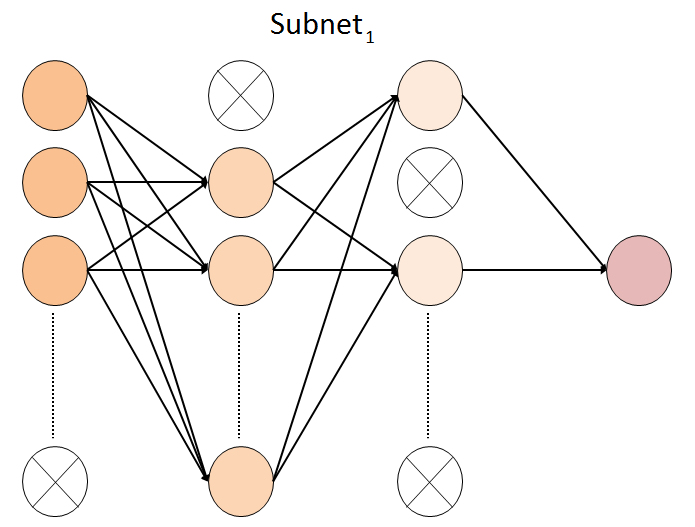
\includegraphics{plots/subnet1.png}}
\end{figure}
\end{vbframe}
%%%%%%%%%%%%%%%%%%%%%%%%%%%%%%%%%%%%%%%%%%%%%%%%%%%%%%%%%%%%%%%%%%

\endlecture
\end{document}
